% Copyright 2006 by Till Tantau
%
% This file may be distributed and/or modified
%
% 1. under the LaTeX Project Public License and/or
% 2. under the GNU Free Documentation License.
%
% See the file doc/generic/pgf/licenses/LICENSE for more details.


\section{Constructing Paths}

\subsection{Overview}

The ``basic entity of drawing'' in \pgfname\ is the \emph{path}. A
path consists of several parts, each of which is either a closed or
open curve. An open curve has a starting point and an end point and,
in between, consists of several \emph{segments}, each of which is
either a straight line or a B\'ezier curve. Here is an example of a
path (in red) consisting of two parts, one open, one closed:

\begin{codeexample}[]
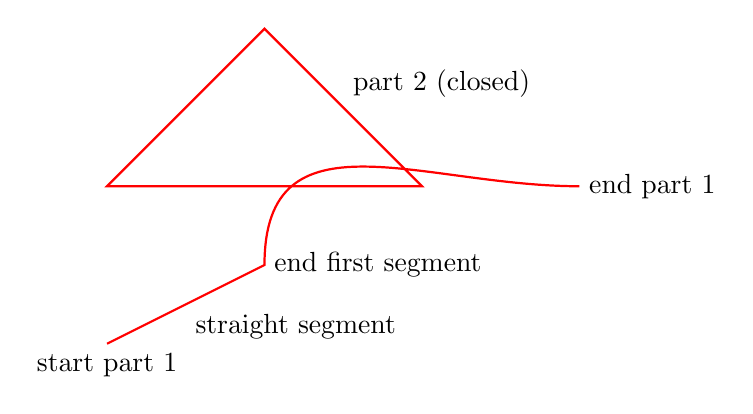
\begin{tikzpicture}[scale=2]
  \draw[thick,red]
       (0,0) coordinate (a)
    -- coordinate (ab) (1,.5) coordinate (b)
    .. coordinate (bc) controls +(up:1cm) and +(left:1cm) .. (3,1)  coordinate (c)
       (0,1) -- (2,1) -- coordinate (x) (1,2) -- cycle;

  \draw (a)  node[below] {start part 1}
        (ab) node[below right] {straight segment}
        (b)  node[right] {end first segment}
        (c)  node[right] {end part 1}
        (x)  node[above right]  {part 2 (closed)};
\end{tikzpicture}
\end{codeexample}

A path, by itself, has no ``effect,'' that is, it does not leave any
marks on the page. It is just a set of points on the plane. However,
you can \emph{use} a path in different ways. The most natural actions
are \emph{stroking} (also known as \emph{drawing}) and
\emph{filling}. Stroking can be imagined as picking up a pen of a
certain diameter and ``moving it along the path.'' Filling means that
everything ``inside'' the path is filled with a uniform
color. Naturally, the open parts of a path must first be closed before
a path can be filled.

In \pgfname, there are numerous commands for constructing paths, all
of which start with |\pgfpath|. There are also commands for
\emph{using} paths, though most operations can be performed by calling
|\pgfusepath| with an appropriate parameter.

As a side-effect, the path construction commands keep track of two
bounding boxes. One is the bounding box for the current path, the
other is a bounding box for all paths in the current picture. See
Section~\ref{section-bb} for more details.

Each path construction command extends the current path in some
way. The ``current path'' is a global entity that persists across
\TeX\ groups. Thus, between calls to the path construction commands
you can perform arbitrary computations and even open and closed \TeX\
groups. The current path only gets ``flushed'' when the |\pgfusepath|
command is called (or when the soft-path subsystem is used directly,
see Section~\ref{section-soft-paths}).

\subsection{The Move-To Path Operation}

The most basic operation is the move-to operation. It must be given at
the beginning of paths, though some path construction command (like
|\pgfpathrectangle|) generate move-tos implicitly. A move-to operation
can also be used to start a new part of a path.

\begin{command}{\pgfpathmoveto\marg{coordinate}}
  This command expects a \pgfname-coordinate like |\pgfpointorigin| as
  its parameter. When the current path is empty, this operation will
  start the path at the given \meta{coordinate}. If a path has already
  been partly constructed, this command will end the current part of
  the path and start a new one.
\begin{codeexample}[]
\begin{pgfpicture}
  \pgfpathmoveto{\pgfpointorigin}
  \pgfpathlineto{\pgfpoint{1cm}{1cm}}
  \pgfpathlineto{\pgfpoint{2cm}{1cm}}
  \pgfpathlineto{\pgfpoint{3cm}{0.5cm}}
  \pgfpathlineto{\pgfpoint{3cm}{0cm}}
  \pgfsetfillcolor{examplefill}
  \pgfusepath{fill,stroke}
\end{pgfpicture}
\end{codeexample}
\begin{codeexample}[]
\begin{pgfpicture}
  \pgfpathmoveto{\pgfpointorigin}
  \pgfpathlineto{\pgfpoint{1cm}{1cm}}
  \pgfpathlineto{\pgfpoint{2cm}{1cm}}
  \pgfpathmoveto{\pgfpoint{2cm}{1cm}} % New part
  \pgfpathlineto{\pgfpoint{3cm}{0.5cm}}
  \pgfpathlineto{\pgfpoint{3cm}{0cm}}
  \pgfsetfillcolor{examplefill}
  \pgfusepath{fill,stroke}
\end{pgfpicture}
\end{codeexample}
  The command will apply the current coordinate transformation matrix
  to \meta{coordinate} before using it.

  The command will update the bounding box of the current path and
  picture, if necessary.
\end{command}


\subsection{The Line-To Path Operation}

\begin{command}{\pgfpathlineto\marg{coordinate}}
  This command extends the current path in a straight line to the
  given \meta{coordinate}. If this command is given at the beginning
  of path without any other path construction command given before (in
  particular without a move-to operation), the \TeX\ file may compile
  without an error message, but a viewer application may display an
  error message when trying to render the picture.
\begin{codeexample}[]
\begin{pgfpicture}
  \pgfpathmoveto{\pgfpointorigin}
  \pgfpathlineto{\pgfpoint{1cm}{1cm}}
  \pgfpathlineto{\pgfpoint{2cm}{1cm}}
  \pgfsetfillcolor{examplefill}
  \pgfusepath{fill,stroke}
\end{pgfpicture}
\end{codeexample}
  The command will apply the current coordinate transformation matrix
  to \meta{coordinate} before using it.

  The command will update the bounding box of the current path and
  picture, if necessary.
\end{command}


\subsection{The Curve-To Path Operations}

\begin{command}{\pgfpathcurveto\marg{support 1}\marg{support 2}\marg{coordinate}}
  This command extends the current path with a B\'ezier curve from the
  last point of the path to  \meta{coordinate}. The \meta{support 1}
  and \meta{support 2} are the first and second support point of the
  B\'ezier curve. For more information on B\'ezier curve, please consult a
  standard textbook on computer graphics.

  Like the line-to command, this command may not be the first path
  construction command in a path.
\begin{codeexample}[]
\begin{pgfpicture}
  \pgfpathmoveto{\pgfpointorigin}
  \pgfpathcurveto
    {\pgfpoint{1cm}{1cm}}{\pgfpoint{2cm}{1cm}}{\pgfpoint{3cm}{0cm}}
  \pgfsetfillcolor{examplefill}
  \pgfusepath{fill,stroke}
\end{pgfpicture}
\end{codeexample}
  The command will apply the current coordinate transformation matrix
  to \meta{coordinate} before using it.

  The command will update the bounding box of the current path and
  picture, if necessary. However, the bounding box is simply made
  large enough such that it encompasses all of the support points and
  the \meta{coordinate}. This will guarantee that the curve is
  completely inside the bounding box, but the bounding box will
  typically be quite a bit too large. It is not clear (to me) how this
  can be avoided without resorting to ``some serious math'' in order
  to calculate a precise bounding box.
\end{command}

\begin{command}{\pgfpathquadraticcurveto\marg{support}\marg{coordinate}}
  This command works like |\pgfpathcurveto|, only it uses a quadratic
  B\'ezier curve rather than a cubic one. This means that only one
  support point is needed.
\begin{codeexample}[]
\begin{pgfpicture}
  \pgfpathmoveto{\pgfpointorigin}
  \pgfpathquadraticcurveto
    {\pgfpoint{1cm}{1cm}}{\pgfpoint{2cm}{0cm}}
  \pgfsetfillcolor{examplefill}
  \pgfusepath{fill,stroke}
\end{pgfpicture}
\end{codeexample}
  Internally, the quadratic curve is converted into a cubic
  curve. The only noticeable effect of this is that the points used for
  computing the bounding box are the control points of the converted
  curve rather than \meta{support}. The main effect of this is that
  the bounding box will be a bit tighter than might be expected. In
  particular, \meta{support} will not always be part of the bounding
  box.
\end{command}


There exist two commands to draw only part of a cubic B\'ezier curve:

\begin{command}{\pgfpathcurvebetweentime\marg{time $t_1$}\marg{time $t_2$}\marg{point p}\marg{point $s_1$}\marg{point $s_2$}\marg{point q}}

  This command draws the part of the curve described by $p$, $s_1$,
  $s_2$ and $q$ between the times $t_1$ and $t_2$. A time value of 0
  indicates the point $p$ and a time value of 1 indicates point $q$.
  This command includes a moveto operation to the first point.

\begin{codeexample}[]
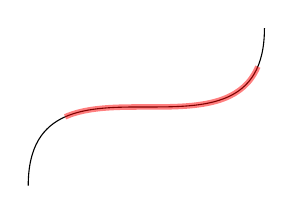
\begin{tikzpicture}
  \draw [thin] (0,0) .. controls (0,2) and (3,0) .. (3,2);
  \pgfpathcurvebetweentime{0.25}{0.9}{\pgfpointxy{0}{0}}{\pgfpointxy{0}{2}}
    {\pgfpointxy{3}{0}}{\pgfpointxy{3}{2}}
  \pgfsetstrokecolor{red}
  \pgfsetstrokeopacity{0.5}
  \pgfsetlinewidth{2pt}
  \pgfusepath{stroke}
\end{tikzpicture}
\end{codeexample}
\end{command}

\begin{command}{\pgfpathcurvebetweentimecontinue\marg{time $t_1$}\marg{time $t_2$}\marg{point p}\marg{point $s_1$}\marg{point $s_2$}\marg{point q}}
  This command works like |\pgfpathcurvebetweentime|, except that a
  moveto operation is \emph{not} made to the first point.
\end{command}


\subsection{The Close Path Operation}

\begin{command}{\pgfpathclose}
  This command closes the current part of the path by appending a
  straight line to the start point of the current part. Note that there
  \emph{is} a difference between closing a path and using the line-to
  operation to add a straight line to the start of the current
  path. The difference is demonstrated by the upper corners of the triangles
  in the following example:
\begin{codeexample}[]
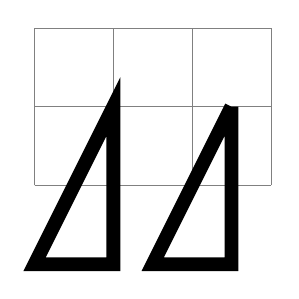
\begin{tikzpicture}
  \draw[help lines] (0,0) grid (3,2);
  \pgfsetlinewidth{5pt}
  \pgfpathmoveto{\pgfpoint{1cm}{1cm}}
  \pgfpathlineto{\pgfpoint{0cm}{-1cm}}
  \pgfpathlineto{\pgfpoint{1cm}{-1cm}}
  \pgfpathclose
  \pgfpathmoveto{\pgfpoint{2.5cm}{1cm}}
  \pgfpathlineto{\pgfpoint{1.5cm}{-1cm}}
  \pgfpathlineto{\pgfpoint{2.5cm}{-1cm}}
  \pgfpathlineto{\pgfpoint{2.5cm}{1cm}}
  \pgfusepath{stroke}
\end{tikzpicture}
\end{codeexample}
\end{command}


\subsection{Arc, Ellipse and Circle Path Operations}

The path construction commands that we have discussed up to now are
sufficient to create all paths that can be created ``at all.''
However, it is useful to have special commands to create certain
shapes, like circles, that arise often in practice.

In the following, the commands for adding (parts of) (transformed)
circles to a path are described.

\begin{command}{\pgfpatharc\marg{start angle}\marg{end
      angle}{\ttfamily\char`\{}\meta{radius}\opt{| and |\meta{y-radius}}{\ttfamily\char`\}}}
  This command appends a part of a circle (or an ellipse) to the current
  path. Imaging the curve between \meta{start angle} and \meta{end
    angle} on a circle of radius \meta{radius} (if $\meta{start angle}
  < \meta{end angle}$, the curve goes around the circle
  counterclockwise, otherwise clockwise). This curve is now moved such
  that the point where the curve starts is the previous last point of the
  path. Note that this command will \emph{not} start a new part of the
  path, which is important for example for filling purposes.

\begin{codeexample}[]
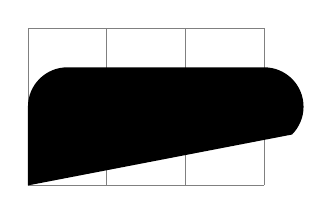
\begin{tikzpicture}
  \draw[help lines] (0,0) grid (3,2);
  \pgfpathmoveto{\pgfpointorigin}
  \pgfpathlineto{\pgfpoint{0cm}{1cm}}
  \pgfpatharc{180}{90}{.5cm}
  \pgfpathlineto{\pgfpoint{3cm}{1.5cm}}
  \pgfpatharc{90}{-45}{.5cm}
  \pgfusepath{fill}
\end{tikzpicture}
\end{codeexample}

  Saying |\pgfpatharc{0}{360}{1cm}| ``nearly'' gives you a full
  circle. The ``nearly'' refers to the fact that the circle will not
  be closed. You can close it using |\pgfpathclose|.

  If the optional \meta{y-radius} is given, the \meta{radius} is the
  $x$-radius and the \meta{y-radius} the $y$-radius of the ellipse
  from which the curve is taken:

\begin{codeexample}[]
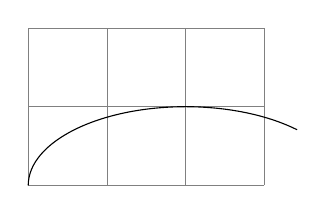
\begin{tikzpicture}
  \draw[help lines] (0,0) grid (3,2);
  \pgfpathmoveto{\pgfpointorigin}
  \pgfpatharc{180}{45}{2cm and 1cm}
  \pgfusepath{draw}
\end{tikzpicture}
\end{codeexample}

  The axes of the circle or ellipse from which the arc is ``taken''
  always point up and right. However, the current coordinate
  transformation matrix will have an effect on the arc. This can be
  used to, say, rotate an arc:

\begin{codeexample}[]
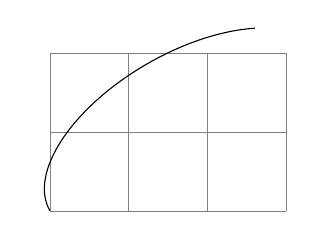
\begin{tikzpicture}
  \draw[help lines] (0,0) grid (3,2);
  \pgftransformrotate{30}
  \pgfpathmoveto{\pgfpointorigin}
  \pgfpatharc{180}{45}{2cm and 1cm}
  \pgfusepath{draw}
\end{tikzpicture}
\end{codeexample}

  The command will update the bounding box of the current path and
  picture, if necessary. Unless rotation or shearing transformations
  are applied, the bounding box will be tight.
\end{command}

\begin{command}{\pgfpatharcaxes\marg{start angle}\marg{end
      angle}\marg{first axis}\marg{second axis}}
  This command is similar to |\pgfpatharc|. The main difference is how
  the ellipse or circle is specified from which the arc is taken. The
  two parameters \meta{first axis} and \meta{second axis} are the
  $0^\circ$-axis and the $90^\circ$-axis of the ellipse from which the
  path is taken. Thus, |\pgfpatharc{0}{90}{1cm and 2cm}| has the same effect
  as
\begin{verbatim}
\pgfpatharcaxes{0}{90}{\pgfpoint{1cm}{0cm}}{\pgfpoint{0cm}{2cm}}
\end{verbatim}
\begin{codeexample}[]
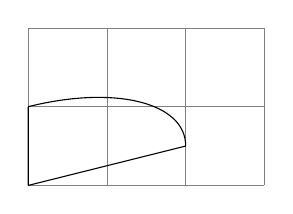
\begin{tikzpicture}
  \draw[help lines] (0,0) grid (3,2);
  \draw (0,0) -- (2cm,5mm) (0,0) -- (0cm,1cm);

  \pgfpathmoveto{\pgfpoint{2cm}{5mm}}
  \pgfpatharcaxes{0}{90}{\pgfpoint{2cm}{5mm}}{\pgfpoint{0cm}{1cm}}
  \pgfusepath{draw}
\end{tikzpicture}
\end{codeexample}
\end{command}


\begin{command}{\pgfpatharcto\marg{x-radius}\marg{y-radius}\marg{rotation}
    \marg{large arc flag}\marg{counterclockwise flag}\\\marg{target point}}
  This command (which directly corresponds to the arc-path command of
  \textsc{svg}) is used to add an arc to the path that starts at the
  current point and ends at \meta{target point}. This arc is part of
  an ellipse that is determined in the following way: Imagine an
  ellipse with radii \meta{x-radius} and \meta{y-radius} that is
  rotated around its center by \meta{rotation} degrees. When you move
  this ellipse around in the plane, there will be exactly two
  positions such that the two current point and the target point lie
  on the border of the ellipse (excluding pathological cases). The
  flags \meta{large arc flag} and \meta{clockwise flag} are then used to
  decide which of these ellipses should be picked and which arc on the
  picked ellipsis should be used.
\begin{codeexample}[]
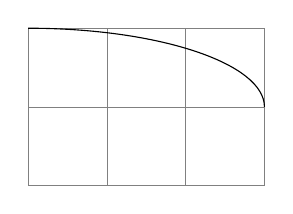
\begin{tikzpicture}
  \draw[help lines] (0,0) grid (3,2);

  \pgfpathmoveto{\pgfpoint{0mm}{20mm}}
  \pgfpatharcto{3cm}{1cm}{0}{0}{0}{\pgfpoint{3cm}{1cm}}
  \pgfusepath{draw}
\end{tikzpicture}
\end{codeexample}
  Both flags are considered to be false exactly if they evaluate to
  |0|, otherwise they are true. If the \meta{large arc flag} is true,
  then the angle spanned by the arc will be greater than $180^\circ$,
  otherwise it will be less than $180^\circ$. The \meta{clockwise
    flag} is used to determine which of the two ellipses should be
  used: if the flag is true, then the arc goes from the current point
  to the target point in a counterclockwise direction, otherwise in a
  clockwise fashion.
\begin{codeexample}[]
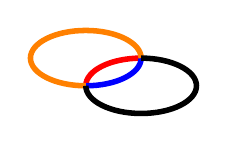
\begin{tikzpicture}
  \pgfsetlinewidth{2pt}
  % Flags 0 0: red
  \pgfsetstrokecolor{red}
  \pgfpathmoveto{\pgfpointorigin}
  \pgfpatharcto{20pt}{10pt}{0}{0}{0}{\pgfpoint{20pt}{10pt}}
  \pgfusepath{stroke}
  % Flags 0 1: blue
  \pgfsetstrokecolor{blue}
  \pgfpathmoveto{\pgfpointorigin}
  \pgfpatharcto{20pt}{10pt}{0}{0}{1}{\pgfpoint{20pt}{10pt}}
  \pgfusepath{stroke}
  % Flags 1 0: orange
  \pgfsetstrokecolor{orange}
  \pgfpathmoveto{\pgfpointorigin}
  \pgfpatharcto{20pt}{10pt}{0}{1}{0}{\pgfpoint{20pt}{10pt}}
  \pgfusepath{stroke}
  % Flags 1 1: black
  \pgfsetstrokecolor{black}
  \pgfpathmoveto{\pgfpointorigin}
  \pgfpatharcto{20pt}{10pt}{0}{1}{1}{\pgfpoint{20pt}{10pt}}
  \pgfusepath{stroke}
\end{tikzpicture}
\end{codeexample}
  \emph{Warning:} The internal computations necessary for this command
  are numerically very unstable. In particular, the arc will not
  always really end at the \meta{target coordinate}, but may be off by
  up to several points. A more precise positioning is currently
  infeasible due to \TeX's numerical weaknesses. The only case that
  works quite nicely is when the resulting angle is a multiple
  of~$90^\circ$.
\end{command}

\begin{command}{\pgfpatharctoprecomputed\marg{center point}\marg{start angle}\marg{end angle}\marg{end point}\\\marg{x-radius}\marg{y-radius}\marg{ratio x-radius/y-radius}\marg{ratio y-radius/x-radius}}
	A specialized arc operation which is fast and numerically stable, provided a lot of information is given in advance.

	In contrast to |\pgfpatharc|, it explicitly interpolates start- and end points.

	In contrast to |\pgfpatharcto|, this routine is numerically stable and quite fast since it relies on a lot of available information.
\begin{codeexample}[]
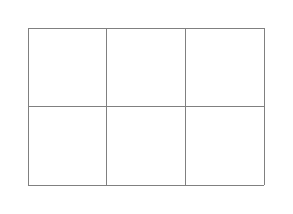
\begin{tikzpicture}
  \draw[help lines] (0,0) grid (3,2);

  \def\cx{1.5cm}% center x
  \def\cy{1cm}% center y
  \def\startangle{0}%
  \def\endangle{270}%
  \def\a{1.5cm}% xradius
  \def\b{0.5cm}% yradius
  \pgfmathparse{\a/\b}\let\abratio=\pgfmathresult
  \pgfmathparse{\b/\a}\let\baratio=\pgfmathresult
  %
  % start point:
  \pgfpathmoveto{\pgfpoint{\cx+\a*cos(\startangle)}{\cy+\b*sin(\startangle)}}%
  \pgfpatharctoprecomputed
    {\pgfpoint{\cx}{\cy}}
    {\startangle}
    {\endangle}
    {\pgfpoint{\cx+\a*cos(\endangle)}{\cy+\b*sin(\endangle)}}% end point
    {\a}
    {\b}
    {\abratio}
    {\baratio}
  \pgfusepath{draw}
\end{tikzpicture}
\end{codeexample}

  	\begin{command}{\pgfpatharctomaxstepsize}
          The quality of arc approximation taken by
          |\pgfpatharctoprecomputed| by means of B\'ezier splines is
          controlled by a mesh width, which is initially

	|\def\pgfpatharctoprecomputed{45}|.

	The mesh width is provided in (full!) degrees. The smaller the mesh
	width, the more precise the arc approximation.

	Use an empty value to disable spline approximation (uses a single
	cubic polynomial for the complete arc).

	The value must be an integer!
	\end{command}
\end{command}

\begin{command}{\pgfpathellipse\marg{center}\marg{first
      axis}\marg{second axis}}
  The effect of this command is to append an ellipse to the current
  path (if the path is not empty, a new part is started). The
  ellipse's center will be \meta{center} and \meta{first axis} and
  \meta{second axis} are the axis \emph{vectors}. The same effect as
  this command can also be achieved using an appropriate sequence of
  move-to, arc, and close operations, but this command is easier and
  faster.

\begin{codeexample}[]
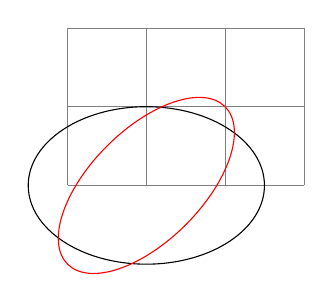
\begin{tikzpicture}
  \draw[help lines] (0,0) grid (3,2);
  \pgfpathellipse{\pgfpoint{1cm}{0cm}}
                 {\pgfpoint{1.5cm}{0cm}}
                 {\pgfpoint{0cm}{1cm}}
  \pgfusepath{draw}
  \color{red}
  \pgfpathellipse{\pgfpoint{1cm}{0cm}}
                 {\pgfpoint{1cm}{1cm}}
                 {\pgfpoint{-0.5cm}{0.5cm}}
  \pgfusepath{draw}
\end{tikzpicture}
\end{codeexample}

  The command will apply coordinate transformations to all coordinates
  of the ellipse. However, the coordinate transformations are applied
  only after the ellipse is ``finished conceptually.'' Thus, a
  transformation of 1cm to the right will simply shift the ellipse one
  centimeter to the right; it will not add 1cm to the $x$-coordinates
  of the two axis vectors.

  The command will update the bounding box of the current path and
  picture, if necessary.
\end{command}

\begin{command}{\pgfpathcircle\marg{center}\marg{radius}}
  A shorthand for |\pgfpathellipse| applied to \meta{center} and the
  two axis vectors $(\meta{radius},0)$ and $(0,\meta{radius})$.
\end{command}


\subsection{Rectangle Path Operations}

Another shape that arises frequently is the rectangle. Two commands
can be used to add a rectangle to the current path. Both commands will
start a new part of the path.


\begin{command}{\pgfpathrectangle\marg{corner}\marg{diagonal vector}}
  Adds a rectangle to the path whose one corner is \meta{corner} and
  whose opposite corner is given by $\meta{corner} + \meta{diagonal
    vector}$.

\begin{codeexample}[]
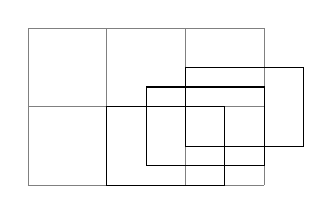
\begin{tikzpicture}
  \draw[help lines] (0,0) grid (3,2);
  \pgfpathrectangle{\pgfpoint{1cm}{0cm}}{\pgfpoint{1.5cm}{1cm}}
  \pgfpathrectangle{\pgfpoint{1.5cm}{0.25cm}}{\pgfpoint{1.5cm}{1cm}}
  \pgfpathrectangle{\pgfpoint{2cm}{0.5cm}}{\pgfpoint{1.5cm}{1cm}}
  \pgfusepath{draw}
\end{tikzpicture}
\end{codeexample}
  The command will apply coordinate transformations and update the
  bounding boxes tightly.
\end{command}


\begin{command}{\pgfpathrectanglecorners\marg{corner}\marg{opposite corner}}
  Adds a rectangle to the path whose two opposing corners are
  \meta{corner} and \meta{opposite corner}.
\begin{codeexample}[]
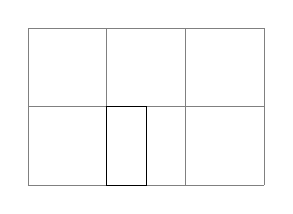
\begin{tikzpicture}
  \draw[help lines] (0,0) grid (3,2);
  \pgfpathrectanglecorners{\pgfpoint{1cm}{0cm}}{\pgfpoint{1.5cm}{1cm}}
  \pgfusepath{draw}
\end{tikzpicture}
\end{codeexample}
  The command will apply coordinate transformations and update the
  bounding boxes tightly.
\end{command}



\subsection{The Grid Path Operation}

\begin{command}{\pgfpathgrid\oarg{options}\marg{lower left}\marg{upper right}}
  Appends a grid to the current path. That is, a (possibly large)
  number of parts are added to the path, each part consisting of a
  single horizontal or vertical straight line segment.

  Conceptually, the origin is part of the grid and the grid is clipped
  to the rectangle specified by the \meta{lower left} and
  the \meta{upper right} corner. However, no clipping occurs (this
  command just adds parts to the current path). Rather, the points
  where the lines enter and leave the ``clipping area'' are computed
  and used to add simple lines to the current path.

  The following keys influence the grid:
  \begin{key}{/pgf/stepx=\meta{dimension} (initially 1cm)}
    The horizontal stepping.
  \end{key}
  \begin{key}{/pgf/stepy=\meta{dimension} (initially 1cm)}
    The vertical stepping.
  \end{key}
  \begin{key}{/pgf/step=\meta{vector}}
    Sets the horizontal stepping to the $x$-coordinate of
    \meta{vector} and the vertical stepping to its $y$-coordinate.
  \end{key}
\begin{codeexample}[]
\begin{pgfpicture}
  \pgfsetlinewidth{0.8pt}
  \pgfpathgrid[step={\pgfpoint{1cm}{1cm}}]
    {\pgfpoint{-3mm}{-3mm}}{\pgfpoint{33mm}{23mm}}
  \pgfusepath{stroke}
  \pgfsetlinewidth{0.4pt}
  \pgfpathgrid[stepx=1mm,stepy=1mm]
    {\pgfpoint{-1.5mm}{-1.5mm}}{\pgfpoint{31.5mm}{21.5mm}}
  \pgfusepath{stroke}
\end{pgfpicture}
\end{codeexample}
  The command will apply coordinate transformations and update the
  bounding boxes tightly. As for ellipses, the transformations are
  applied to the ``conceptually finished'' grid.
\begin{codeexample}[]
\begin{pgfpicture}
  \pgftransformrotate{10}
  \pgfpathgrid[stepx=1mm,stepy=2mm]{\pgfpoint{0mm}{0mm}}{\pgfpoint{30mm}{30mm}}
  \pgfusepath{stroke}
\end{pgfpicture}
\end{codeexample}
\end{command}


\subsection{The Parabola Path Operation}

\begin{command}{\pgfpathparabola\marg{bend vector}\marg{end vector}}
  This command appends two half-parabolas to the  current path. The
  first starts at the current point and ends at the current point plus
  \meta{bend vector}. At his point, it has its bend. The second half
  parabola starts at that bend point and end at point that is given by
  the bend plus \meta{end vector}.

  If you set \meta{end vector} to the null vector, you append only a
  half parabola that goes from the current point to the bend; by
  setting \meta{bend vector} to the null vector, you append only a
  half parabola that goes to current point plus \meta{end vector} and
  has its bend at the current point.

  It is not possible to use this command to draw a part of a parabola
  that does not contain the bend.

\begin{codeexample}[]
\begin{pgfpicture}
  % Half-parabola going ``up and right''
  \pgfpathmoveto{\pgfpointorigin}
  \pgfpathparabola{\pgfpointorigin}{\pgfpoint{2cm}{4cm}}
  \color{red}
  \pgfusepath{stroke}

  % Half-parabola going ``down and right''
  \pgfpathmoveto{\pgfpointorigin}
  \pgfpathparabola{\pgfpoint{-2cm}{4cm}}{\pgfpointorigin}
  \color{blue}
  \pgfusepath{stroke}

  % Full parabola
  \pgfpathmoveto{\pgfpoint{-2cm}{2cm}}
  \pgfpathparabola{\pgfpoint{1cm}{-1cm}}{\pgfpoint{2cm}{4cm}}
  \color{orange}
  \pgfusepath{stroke}
\end{pgfpicture}
\end{codeexample}
  The command will apply coordinate transformations and update the
  bounding boxes.
\end{command}


\subsection{Sine and Cosine Path Operations}

Sine and cosine curves often need to be drawn and the following commands
may help with this. However, they only allow you to append sine and
cosine curves in intervals that are multiples of $\pi/2$.

\begin{command}{\pgfpathsine\marg{vector}}
  This command appends a sine curve in the interval $[0,\pi/2]$ to the
  current path. The sine curve is squeezed or stretched such that the
  curve starts at the current point and ends at the current point plus
  \meta{vector}.
\begin{codeexample}[]
\begin{tikzpicture}
  \draw[help lines] (0,0) grid (3,1);
  \pgfpathmoveto{\pgfpoint{1cm}{0cm}}
  \pgfpathsine{\pgfpoint{1cm}{1cm}}
  \pgfusepath{stroke}

  \color{red}
  \pgfpathmoveto{\pgfpoint{1cm}{0cm}}
  \pgfpathsine{\pgfpoint{-2cm}{-2cm}}
  \pgfusepath{stroke}
\end{tikzpicture}
\end{codeexample}
  The command will apply coordinate transformations and update the
  bounding boxes.
\end{command}

\begin{command}{\pgfpathcosine\marg{vector}}
  This command appends a cosine curve in the interval $[0,\pi/2]$ to the
  current path. The curve is squeezed or stretched such that the
  curve starts at the current point and ends at the current point plus
  \meta{vector}. Using several sine and cosine operations in sequence
  allows you to produce a complete sine or cosine curve
\begin{codeexample}[]
\begin{pgfpicture}
  \pgfpathmoveto{\pgfpoint{0cm}{0cm}}
  \pgfpathsine{\pgfpoint{1cm}{1cm}}
  \pgfpathcosine{\pgfpoint{1cm}{-1cm}}
  \pgfpathsine{\pgfpoint{1cm}{-1cm}}
  \pgfpathcosine{\pgfpoint{1cm}{1cm}}
  \pgfsetfillcolor{examplefill}
  \pgfusepath{fill,stroke}
\end{pgfpicture}
\end{codeexample}
  The command will apply coordinate transformations and update the
  bounding boxes.
\end{command}



\subsection{Plot Path Operations}

There exist several commands for appending
plots to a path. These
commands are available through the module |plot|. They are
documented in Section~\ref{section-plots}.


\subsection{Rounded Corners}

Normally, when you connect two straight line segments or when you
connect two curves that end and start ``at different angles'' you get
``sharp corners'' between the lines or curves. In some cases it is
desirable to produce ``rounded corners'' instead. Thus, the lines
or curves should be shortened a bit and then connected by arcs.

\pgfname\ offers an easy way to achieve this effect, by calling the
following two commands.

\begin{command}{\pgfsetcornersarced\marg{point}}
  This command causes all subsequent corners to be replaced by little
  arcs. The effect of this command lasts till the end of the current
  \TeX\ scope.

  The \meta{point} dictates how large the corner arc will be. Consider
  a corner made by two lines $l$ and~$r$ and assume that the line $l$
  comes first on the path. The $x$-dimension of the \meta{point}
  decides by how much the line~$l$ will be shortened, the
  $y$-dimension of \meta{point} decides by how much the line $r$ will
  be shortened. Then, the shortened lines are connected by an arc.

\begin{codeexample}[]
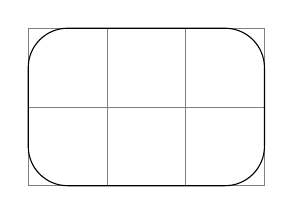
\begin{tikzpicture}
  \draw[help lines] (0,0) grid (3,2);

  \pgfsetcornersarced{\pgfpoint{5mm}{5mm}}
  \pgfpathrectanglecorners{\pgfpointorigin}{\pgfpoint{3cm}{2cm}}
  \pgfusepath{stroke}
\end{tikzpicture}
\end{codeexample}

\begin{codeexample}[]
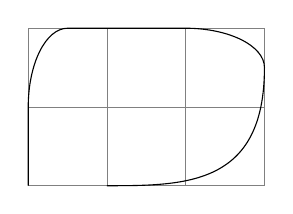
\begin{tikzpicture}
  \draw[help lines] (0,0) grid (3,2);

  \pgfsetcornersarced{\pgfpoint{10mm}{5mm}}
  % 10mm entering,
  % 5mm leaving.
  \pgfpathmoveto{\pgfpointorigin}
  \pgfpathlineto{\pgfpoint{0cm}{2cm}}
  \pgfpathlineto{\pgfpoint{3cm}{2cm}}
  \pgfpathcurveto
    {\pgfpoint{3cm}{0cm}}
    {\pgfpoint{2cm}{0cm}}
    {\pgfpoint{1cm}{0cm}}
  \pgfusepath{stroke}
\end{tikzpicture}
\end{codeexample}

  If the $x$- and $y$-coordinates of \meta{point} are the same and the
  corner is a right angle, you will get a perfect quarter circle
  (well, not quite perfect, but perfect up to six decimals). When the
  angle is not $90^\circ$, you only get a fair approximation.

  More or less ``all'' corners will be rounded, even the corner
  generated by a |\pgfpathclose| command. (The author is a bit proud
  of this feature.)

\begin{codeexample}[]
\begin{pgfpicture}
  \pgfsetcornersarced{\pgfpoint{4pt}{4pt}}
  \pgfpathmoveto{\pgfpointpolar{0}{1cm}}
  \pgfpathlineto{\pgfpointpolar{72}{1cm}}
  \pgfpathlineto{\pgfpointpolar{144}{1cm}}
  \pgfpathlineto{\pgfpointpolar{216}{1cm}}
  \pgfpathlineto{\pgfpointpolar{288}{1cm}}
  \pgfpathclose
  \pgfusepath{stroke}
\end{pgfpicture}
\end{codeexample}

  To return to normal (unrounded) corners, use
  |\pgfsetcornersarced{\pgfpointorigin}|.

  Note that the rounding will produce strange and undesirable effects
  if the lines at the corners are too short. In this case the
  shortening may cause the lines to ``suddenly extend over the other
  end'' which is rarely desirable.
\end{command}




\subsection{Internal Tracking of Bounding Boxes for Paths and Pictures}

\label{section-bb}

\makeatletter

The path construction commands keep track of two bounding boxes: One
for the current path, which is reset whenever the path is used and
thereby flushed, and a bounding box for the current |{pgfpicture}|.

\begin{command}{\pgfresetboundingbox}
	Resets the picture's bounding box. The picture will simply forget any previous bounding box updates and start collecting from scratch.
	
	You can use this together with |\pgfusepath{use as bounding box}| to replace the bounding box by the one of a particular path (ignoring subsequent paths).
\end{command}

The bounding boxes are not accessible by ``normal'' macros. Rather,
two sets of four dimension variables are used for this, all of which
contain the letter~|@|.

\begin{textoken}{\pgf@pathminx}
  The minimum $x$-coordinate ``mentioned'' in the current
  path. Initially, this is set to $16000$pt.
\end{textoken}

\begin{textoken}{\pgf@pathmaxx}
  The maximum $x$-coordinate ``mentioned'' in the current
  path. Initially, this is set to $-16000$pt.
\end{textoken}

\begin{textoken}{\pgf@pathminy}
  The minimum $y$-coordinate ``mentioned'' in the current
  path. Initially, this is set to $16000$pt.
\end{textoken}

\begin{textoken}{\pgf@pathmaxy}
  The maximum $y$-coordinate ``mentioned'' in the current
  path. Initially, this is set to $-16000$pt.
\end{textoken}

\begin{textoken}{\pgf@picminx}
  The minimum $x$-coordinate ``mentioned'' in the current
  picture. Initially, this is set to $16000$pt.
\end{textoken}

\begin{textoken}{\pgf@picmaxx}
  The maximum $x$-coordinate ``mentioned'' in the current
  picture. Initially, this is set to $-16000$pt.
\end{textoken}

\begin{textoken}{\pgf@picminy}
  The minimum $y$-coordinate ``mentioned'' in the current
  picture. Initially, this is set to $16000$pt.
\end{textoken}

\begin{textoken}{\pgf@picmaxy}
  The maximum $y$-coordinate ``mentioned'' in the current
  picture. Initially, this is set to $-16000$pt.
\end{textoken}


Each time a path construction command is called, the above variables
are (globally) updated. To facilitate this, you can use the following
command:

\begin{command}{\pgf@protocolsizes\marg{x-dimension}\marg{y-dimension}}
  Updates all of the above dimension in such a way that the point
  specified by the two arguments is inside both bounding boxes. For
  the picture's bounding box this updating occurs only if
  |\ifpgf@relevantforpicturesize| is true, see below.
\end{command}

For the bounding box of the picture it is not always desirable that
every path construction command affects this bounding box. For
example, if you have just used a clip command, you do not want anything
outside the clipping area to affect the bounding box. For this reason,
there exists a special ``\TeX\ if'' that (locally) decides whether
updating should be applied to the picture's bounding box. Clipping
will set this if to false, as will certain other commands.

\begin{command}{\pgf@relevantforpicturesizefalse}
  Suppresses updating of the picture's bounding box.
\end{command}

\begin{command}{\pgf@relevantforpicturesizetrue}
  Causes updating of the picture's bounding box.
\end{command}
